\chapter{Programmbeschreibung}\label{ch:programmbeschreibung}


\section{Programmablaufplan}\label{sec:pap}

\begin{figure}
    \centering
    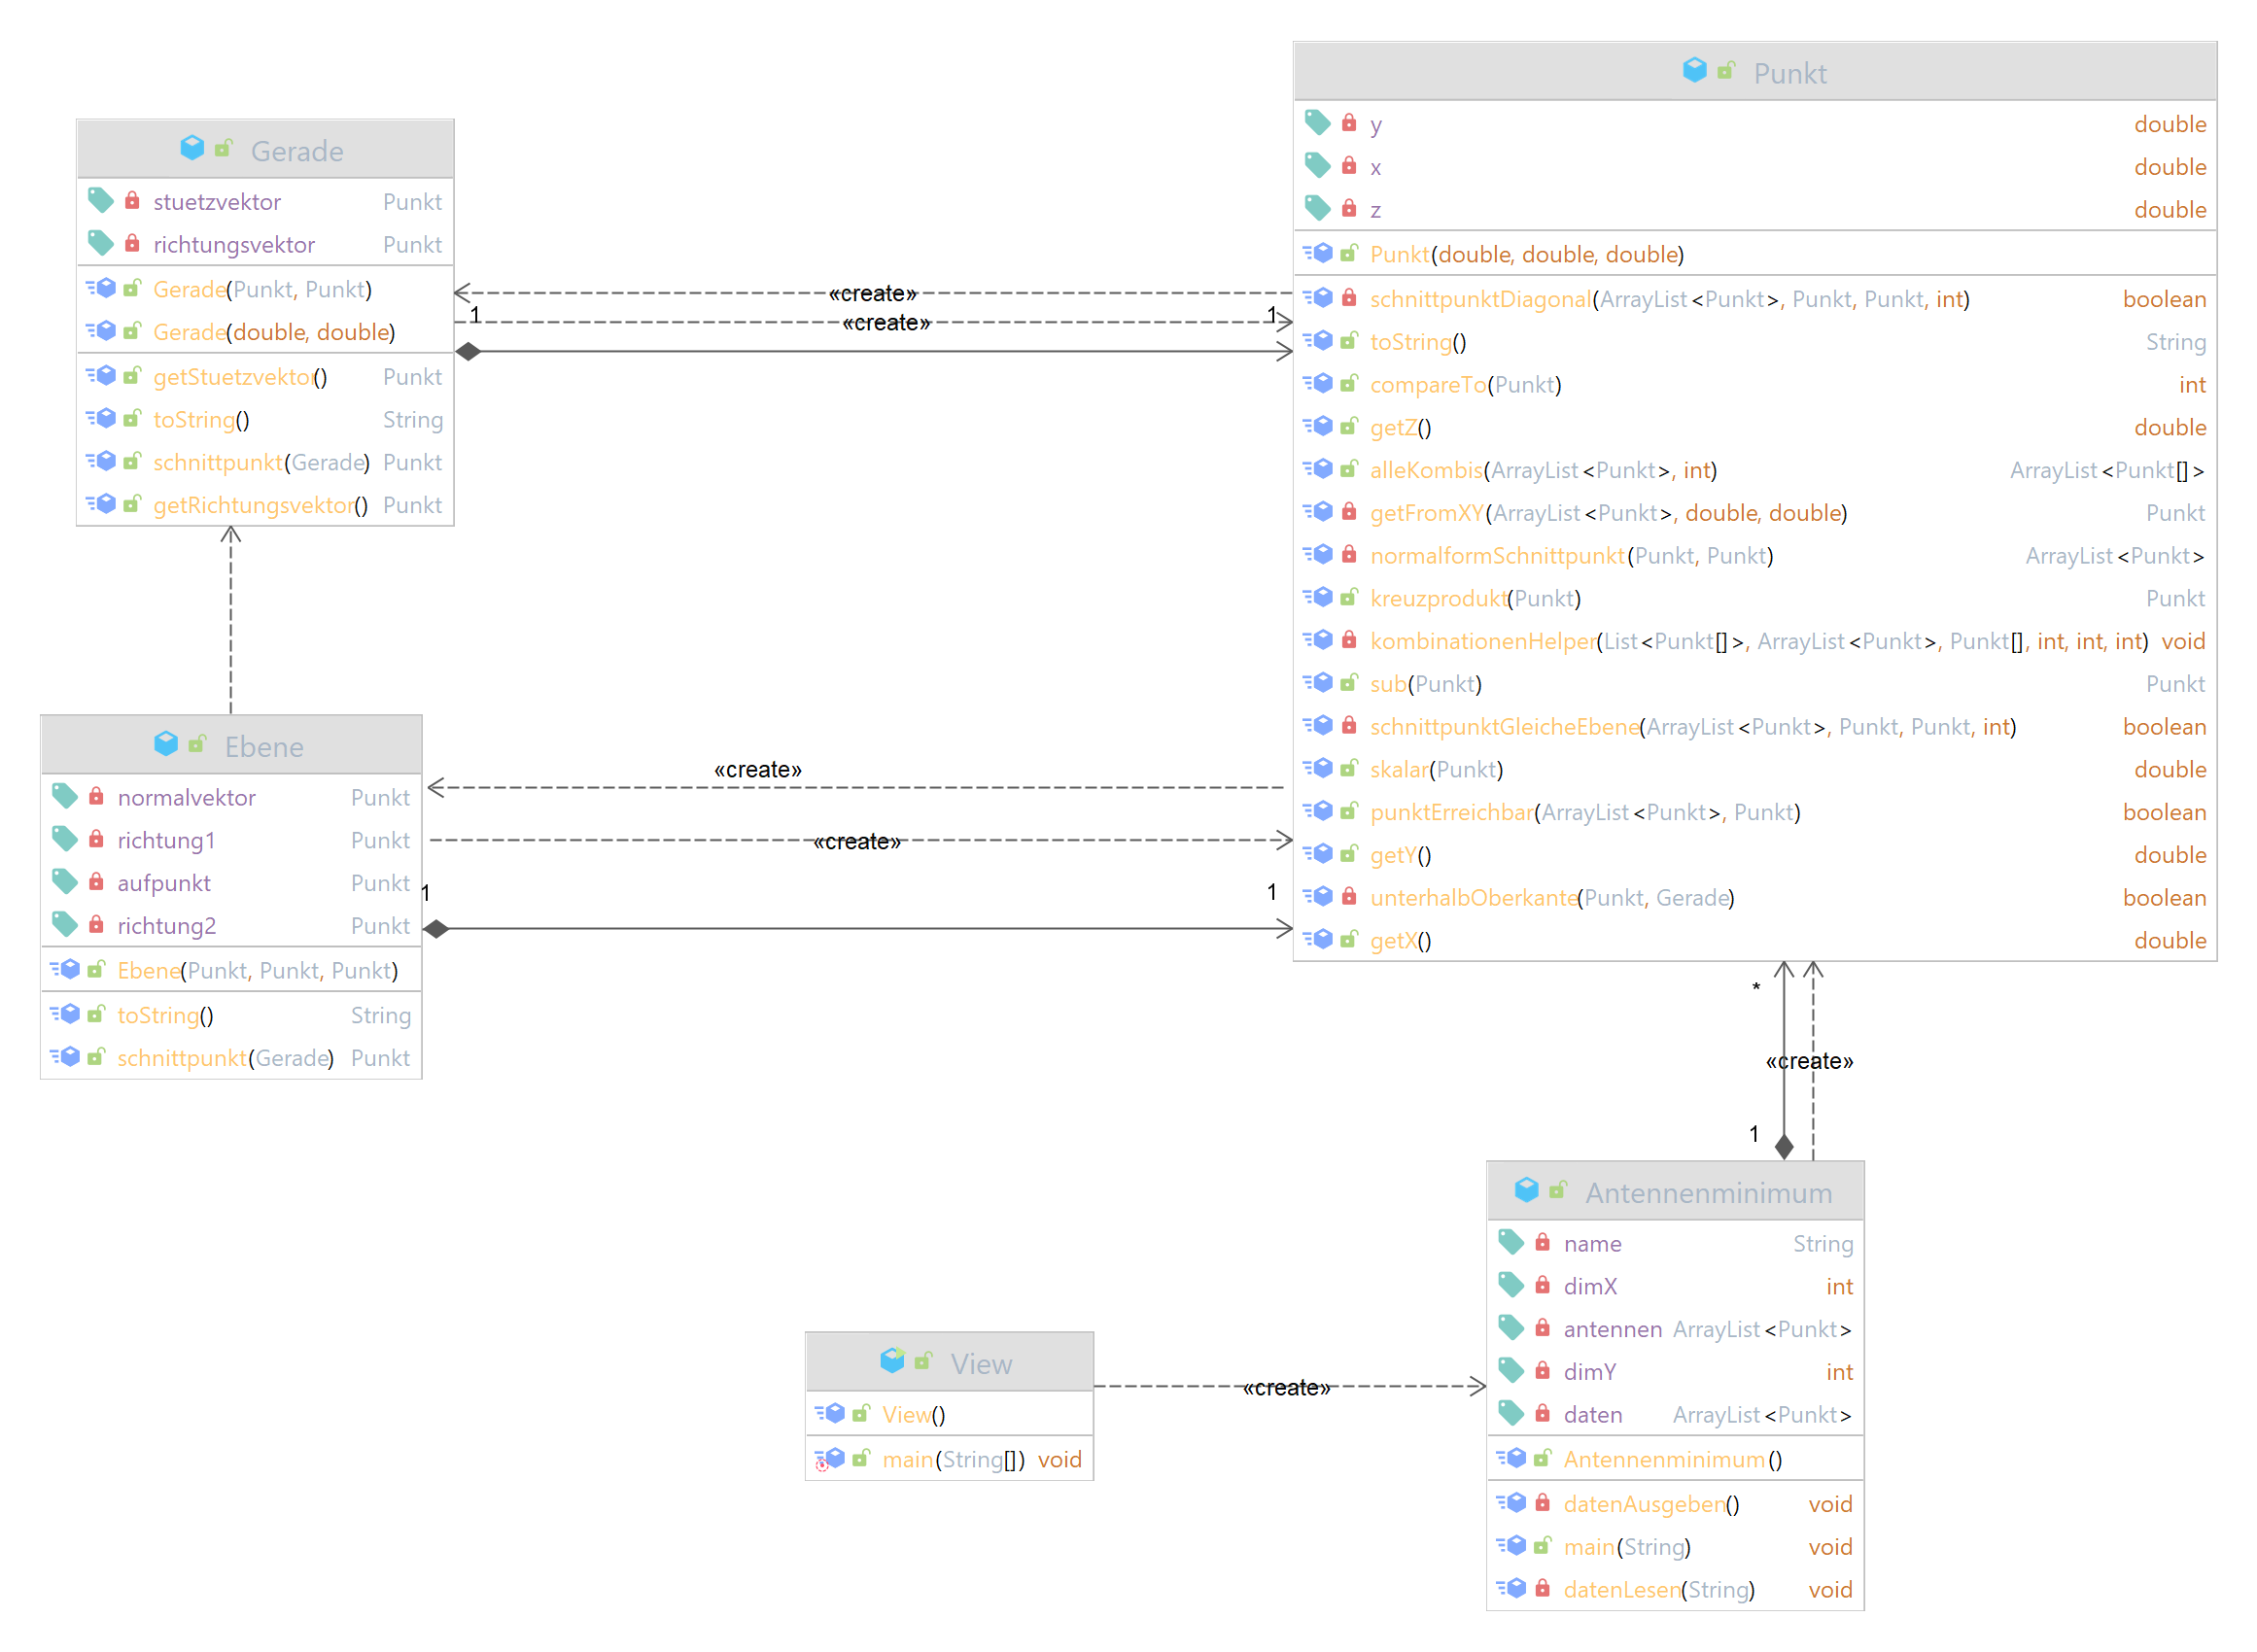
\includegraphics[scale=0.9,width=\textwidth,height=\textheight,keepaspectratio]{class-diagramm-light}
    \caption{Klassendiagramm}
    \label{fig:diagramm1}
\end{figure}

\begin{figure}
    \centering
    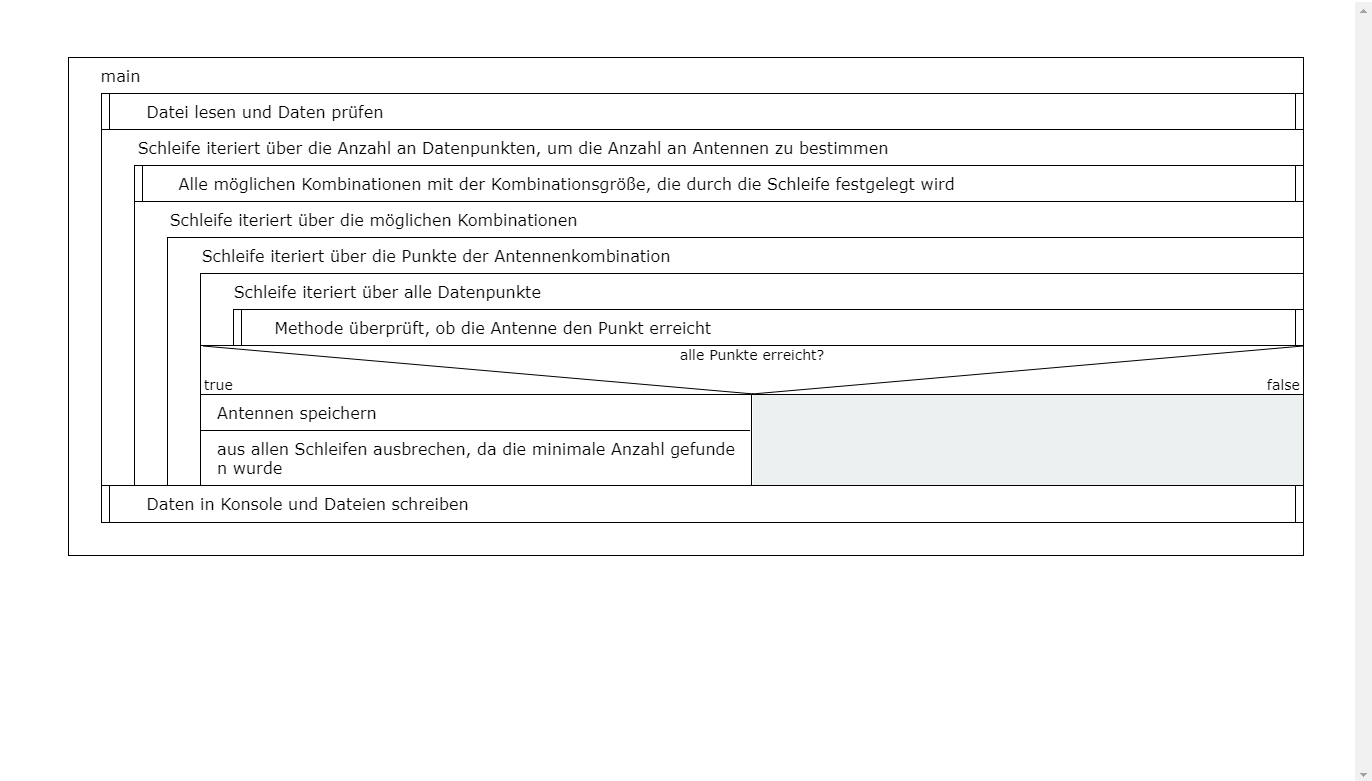
\includegraphics[scale=0.9,width=\textwidth,height=\textheight,keepaspectratio]{struktogramm-main}
    \caption{Struktogramm des Algorithmus}
    \label{fig:diagramm2}
\end{figure}

\begin{figure}[htb]
    \centering
    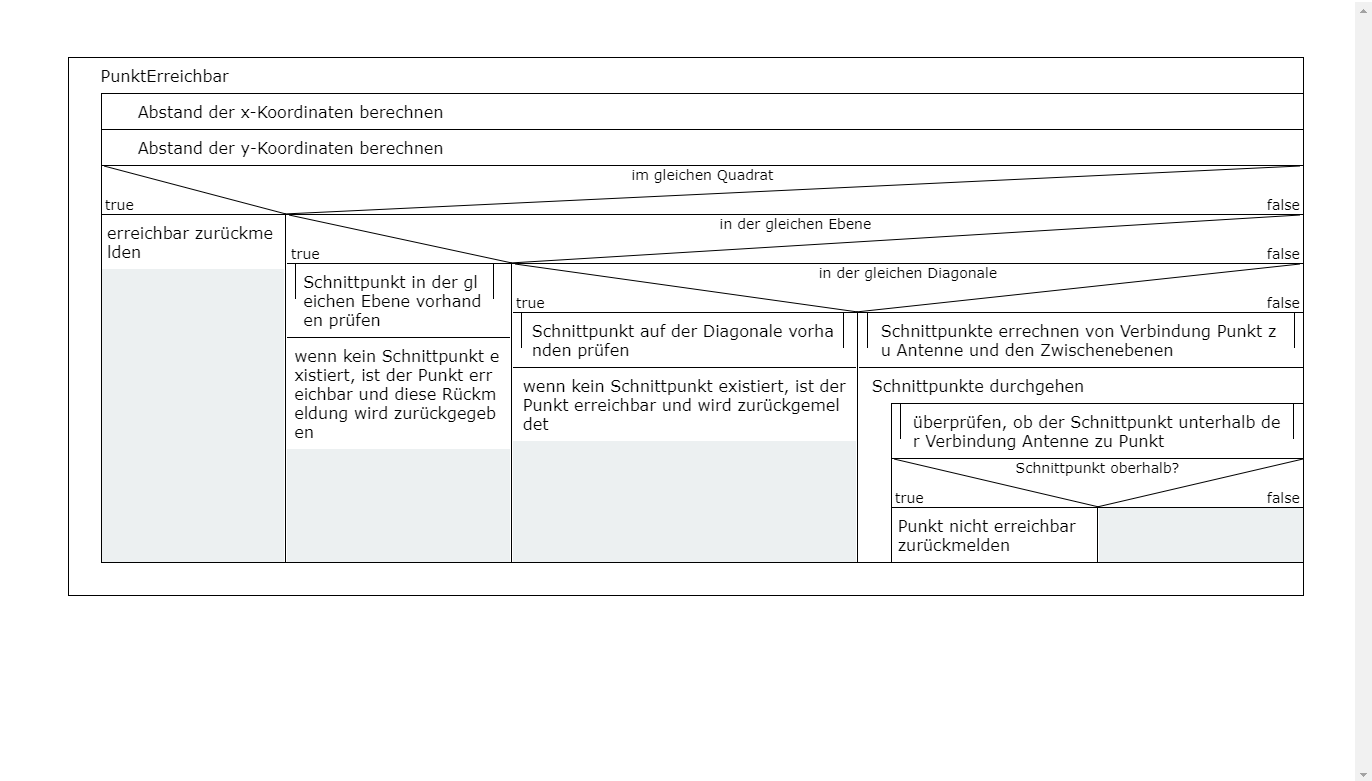
\includegraphics[scale=0.9,width=\textwidth,height=\textheight,keepaspectratio]{struktogramm-punktErreichbar}
    \caption{Struktogramm zur Methode Punkterreichbarkeit prüfen (if-else-Kaskade in Software nicht richtig darstellbar)}
    \label{fig:diagramm3}
\end{figure}



\section{Entwicklungsdokumentation}\label{sec:entwicklerdokumentation}
Im beigefügten Ordner "JavaDoc" ist eine generierte Dokumentation der Methoden zu finden.
\\
Näher zu beschreiben ist die Methode, die überprüft, ob ein Punkt durch eine Antenne erreichbar ist.
Hierbei wird unterteilt in mehrere Bedingung(siehe Struktogramm), zunächst wird geschaut, ob der Punkt im gleichen Quadrat wie die Antenne ist, also direkter Nachbar nach links, rechts, oben, unten oder diagonal ist.
Wenn der Punkt und die Antenne direkte Nachbarn sind, ist der Punkt erreichbar.
Danach wird die Ebene überprüft, das heißt es wird geschaut, ob der Punkt die gleiche x- oder y-Koordinate besitzt.
Dementsprechend wird die Erreichbarkeit geprüft.
Als Nächstes wird geschaut, ob der Punkt in einer direkten Diagonalen zu der Antenne liegt und hierbei auch die Erreichbarkeit.
Wenn diese Bedingungen alle nicht erfüllt werden, wird die letzte Methode aufgerufen, die zu jeder Zwischenebene einen Schnittpunkt errechnet und die Höhe mit der aktuellen Höhe der Verbindung vergleicht.

